\subsubsection{Module 6: Lên lịch và Điều phối}
Module này cung cấp tiện ích giúp người dùng và người bán quản lý thời gian đăng bài hiệu quả, đảm bảo nội dung tiếp cận người xem vào khung giờ vàng.

\begin{figure}[H]
\centering
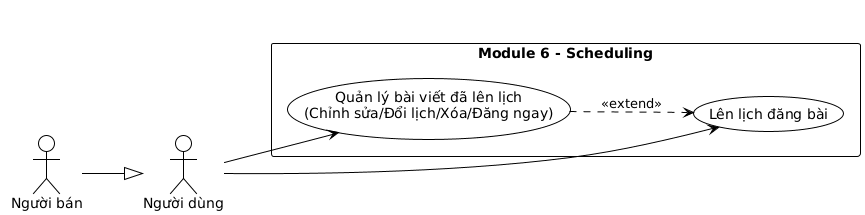
\includegraphics[width=\textwidth]{Images/Usecases/UC-M6-Scheduling.png}
\caption{Sơ đồ Use Case cho Module 6: Lên lịch và Điều phối Bài đăng}
\label{fig:usecase-module6}
\end{figure}

\renewcommand{\arraystretch}{1.3}

% UC6.1: LÊN LỊCH
\begin{table}[H]
\centering
\begin{tabularx}{\textwidth}{|l|X|}
\hline
\textbf{Tên Use Case} & \textbf{UC6.1: Lên lịch đăng bài} \\ \hline
\textbf{Tác nhân} & Người dùng, Người bán \\ \hline
\textbf{Mô tả} & Cung cấp cho người dùng tùy chọn để lên lịch cho một bài đăng, giúp bài viết được tự động xuất bản vào một thời điểm cụ thể trong tương lai. \\ \hline
\textbf{Kích hoạt} & Khi tạo một bài đăng mới, người dùng chọn tùy chọn ``Lên lịch'' thay vì ``Đăng ngay''. \\ \hline
\textbf{Điều kiện tiên quyết} & 
\begin{itemize}
    \item Người dùng đã đăng nhập vào hệ thống.
    \item Người dùng đang ở trong giao diện tạo bài đăng và đã có nội dung cho bài viết.
\end{itemize} \\ \hline
\textbf{Điều kiện sau} & 
\begin{itemize}
    \item Bài đăng được lưu vào cơ sở dữ liệu dưới dạng ``bản nháp đã lên lịch''.
    \item Bài đăng sẽ không hiển thị công khai cho đến đúng thời điểm đã được lên lịch.
\end{itemize} \\ \hline
\textbf{Luồng sự kiện chính} & 
\begin{enumerate}
    \item Trong giao diện tạo bài đăng, sau khi soạn xong nội dung, người dùng chọn tùy chọn ``Lên lịch''.
    \item Một giao diện chọn ngày và giờ trong tương lai sẽ hiện ra.
    \item Người dùng chọn ngày và giờ mong muốn để xuất bản bài viết.
    \item Người dùng nhấn nút ``Xác nhận Lịch''.
    \item Hệ thống lưu bài đăng với trạng thái ``đã lên lịch'' và thời điểm xuất bản đã chọn.
    \item Hệ thống hiển thị thông báo ``Bài viết đã được lên lịch thành công''.
\end{enumerate} \\ \hline
\textbf{Luồng thay thế} & 
\begin{itemize}
    \item A1: Người dùng quyết định không lên lịch nữa và chọn ``Đăng ngay''.
\end{itemize} \\ \hline
\textbf{Ngoại lệ} & 
\begin{itemize}
    \item E1: Người dùng chọn một thời điểm trong quá khứ $\rightarrow$ Hệ thống báo lỗi ``Vui lòng chọn một thời điểm trong tương lai''.
\end{itemize} \\ \hline
\textbf{Ghi chú} & Backend cần có một cơ chế (ví dụ: cron job) để kiểm tra và tự động xuất bản các bài đăng đã đến hạn. \\ \hline
\end{tabularx}
\caption{Đặc tả Use Case Lên lịch đăng bài}
\end{table}

% UC6.2: QUẢN LÝ LỊCH
\begin{table}[H]
\centering
\begin{tabularx}{\textwidth}{|l|X|}
\hline
\textbf{Tên Use Case} & \textbf{UC6.2: Quản lý bài viết đã lên lịch} \\ \hline
\textbf{Tác nhân} & Người dùng, Người bán \\ \hline
\textbf{Mô tả} & Cung cấp một giao diện để người dùng có thể xem lại danh sách các bài viết đang chờ xuất bản, cũng như chỉnh sửa, thay đổi lịch hoặc xóa chúng. \\ \hline
\textbf{Kích hoạt} & Người dùng truy cập vào một mục riêng trong trang cá nhân để xem các bài viết đã lên lịch. \\ \hline
\textbf{Điều kiện tiên quyết} & 
\begin{itemize}
    \item Người dùng đã đăng nhập vào hệ thống.
    \item Người dùng có ít nhất một bài viết đã được lên lịch.
\end{itemize} \\ \hline
\textbf{Điều kiện sau} & Bài viết đã lên lịch được cập nhật (thay đổi nội dung, thời gian) hoặc bị xóa khỏi hàng chờ xuất bản. \\ \hline
\textbf{Luồng sự kiện chính} & 
\begin{enumerate}
    \item Người dùng truy cập vào trang ``Quản lý bài viết đã lên lịch''.
    \item Hệ thống hiển thị danh sách các bài viết đang chờ, kèm theo nội dung xem trước và thời gian dự kiến đăng.
    \item Người dùng chọn một bài viết và thực hiện một trong các hành động: Chỉnh sửa nội dung; Thay đổi lịch; Xóa; Đăng ngay.
    \item Hệ thống cập nhật thay đổi tương ứng vào cơ sở dữ liệu.
\end{enumerate} \\ \hline
\textbf{Luồng thay thế} & 
\begin{itemize}
    \item A1: Người dùng chọn một bài viết và quyết định ``Đăng ngay'' thay vì chờ đến thời gian đã lên lịch.
\end{itemize} \\ \hline
\textbf{Ngoại lệ} & 
\begin{itemize}
    \item E1: Người dùng cố gắng chỉnh sửa một bài viết ngay tại thời điểm nó đang được hệ thống tự động xuất bản $\rightarrow$ Hệ thống báo lỗi hoặc thông báo bài viết đã được đăng.
\end{itemize} \\ \hline
\textbf{Ghi chú} & Giao diện này mang lại sự linh hoạt và quyền kiểm soát hoàn toàn cho người dùng đối với kế hoạch nội dung. \\ \hline
\end{tabularx}
\caption{Đặc tả Use Case Quản lý lịch đăng}
\end{table}